%% ============================================================
%%  Are Prediction Markets Optimal Bayesian Aggregators?
%%  Evidence from 200,000 Polymarket Contracts
%%
%%  Compile: pdflatex main.tex && bibtex main && pdflatex main.tex && pdflatex main.tex
%% ============================================================
\documentclass[12pt,a4paper]{article}

%% -- Packages --
\usepackage[utf8]{inputenc}
\usepackage[T1]{fontenc}
\usepackage{lmodern}
\usepackage{microtype}
\usepackage[margin=2.5cm]{geometry}
\usepackage{amsmath,amssymb,amsthm}
\usepackage{booktabs}
\usepackage{graphicx}
\usepackage{xcolor}
\usepackage{hyperref}
\usepackage{natbib}
\usepackage{setspace}
\usepackage{caption}
\usepackage{subcaption}
\usepackage{float}
\usepackage{array}
\usepackage{multirow}
\usepackage{lineno}
\usepackage{enumitem}
\usepackage[toc,page]{appendix}
\usepackage{siunitx}

%% -- Hyperref setup --
\hypersetup{
  colorlinks = true,
  linkcolor  = blue!70!black,
  citecolor  = blue!70!black,
  urlcolor   = blue!70!black,
  pdftitle   = {Are Prediction Markets Optimal Bayesian Aggregators?},
  pdfauthor  = {},
}

%% -- Theorem environments --
\newtheorem{theorem}{Theorem}[section]
\newtheorem{proposition}[theorem]{Proposition}
\newtheorem{corollary}[theorem]{Corollary}
\theoremstyle{definition}
\newtheorem{definition}[theorem]{Definition}
\theoremstyle{remark}
\newtheorem{remark}[theorem]{Remark}

%% -- Custom commands --
\newcommand{\E}{\mathbb{E}}
\newcommand{\Prob}{\mathbb{P}}
\newcommand{\R}{\mathbb{R}}
\newcommand{\BCI}{\mathrm{BCI}}
\newcommand{\PCD}{\mathrm{PCD}}
\newcommand{\EMH}{\textsc{emh}}
\newcommand{\BME}{\textsc{bme}}
\newcommand{\KL}[2]{D_{\mathrm{KL}}\!\left(#1\,\|\,#2\right)}
\DeclareMathOperator*{\argmin}{arg\,min}

%% -- Spacing --
\onehalfspacing
\setlength{\parskip}{4pt}

%% ============================================================
\begin{document}

%% -- Title page --
\begin{titlepage}
\centering
\vspace*{2cm}

{\LARGE\bfseries Are Prediction Markets Optimal Bayesian Aggregators?\\[0.4em]
Evidence from 200,000 Polymarket Contracts\par}

\vspace{1.5cm}

{\large [Author names removed for blind review]\par}

\vspace{0.8cm}

{\normalsize\itshape
Working Paper — April 2026\par}

\vspace{2cm}

\begin{abstract}
\noindent
We test whether decentralised prediction markets achieve \emph{Bayesian coherence}
--the requirement that the joint probability distribution implied by all related
contract prices satisfies the axioms of probability theory.
Using a cross-sectional snapshot of 200{,}351 contracts on Polymarket (April~2026),
we introduce the \textbf{Partition Coherence Deviation} ($\PCD \equiv \sum_i p_i - 1$),
a market-level measure of how far related-contract prices deviate from exact
probabilistic consistency.
We identify 737 coherence clusters via Polymarket's native event-grouping structure
and classify them as \emph{partition} (single-winner, where coherence requires
$\PCD = 0$) or \emph{non-partition} (multiple winners possible, where $\PCD > 0$
is structurally expected).
For partition clusters, the volume-weighted $\PCD$ is $-4.2\%$, consistent with a
mild but systematic undercounting that generates a risk-free arbitrage opportunity
worth approximately 4 cents per dollar invested across all outcomes.
For non-partition clusters, the volume-weighted $\PCD$ is $+41.3\%$,
with the ten largest violations collectively covering \$60{,}million in contract
volume.
A retrospective longitudinal study over 421 resolved markets shows that
Polymarket \emph{outperforms published superforecaster benchmarks} at all
prediction horizons (Brier 0.128--0.148 vs.\ $\approx$0.15), with accuracy
peaking at T$-$60 days before resolution, consistent with a U-shaped
accuracy-horizon profile driven by short-term speculative noise and
long-horizon irreducible uncertainty.
We propose a unified framework--\textbf{Bayesian Market Efficiency} (\BME)--that
extends the Efficient Market Hypothesis by replacing price-based tests with
probabilistic coherence tests, and show that the standard \EMH\ is nested as a
degenerate special case.
Our results suggest that limits to arbitrage, rather than irrationality, explain
the persistence of coherence violations, with platform risk and coordination costs
as primary frictions.
\end{abstract}

\vspace{1cm}

{\small
\textbf{JEL Codes:} G14, D82, D83, C11\\[4pt]
\textbf{Keywords:} Prediction markets, Bayesian efficiency, probability coherence,
Dutch book, Polymarket, information aggregation, Efficient Market Hypothesis
}
\end{titlepage}

%% ============================================================
\newpage
\tableofcontents
\newpage

%% ============================================================
\section{Introduction}
\label{sec:intro}

The Efficient Market Hypothesis \citep{fama1970} asserts that asset prices fully
reflect all available information.
For traditional financial markets, this claim is tested via price-based
anomalies--momentum, value, calendar effects--and largely survives in
its semi-strong form.
Yet the \EMH\ says nothing about \emph{how} information is aggregated, only that
the final price reflects it.

Prediction markets offer a unique laboratory.
Unlike equity markets, the payoff of a prediction market contract is binary and
precisely defined: \$1 if event $E$ occurs, \$0 otherwise.
Under risk neutrality, the price of this contract at time $t$ is a \emph{direct}
estimate of $\Prob(E \mid \mathcal{I}_t)$, where $\mathcal{I}_t$ is public
information at time $t$.
This makes prediction markets unique among financial instruments: the price
\emph{is} the probability estimate, not a transformed or discounted version of it.

This property allows us to ask a far sharper question than ``are prices right?''
--we can ask: \textbf{are prices Bayesian?}

Bayesian rationality requires more than calibration.
It requires \emph{coherence}: the joint distribution implied by all related
contracts must satisfy the axioms of probability theory.
If market $A$ prices $\Prob(\text{Team X wins}) = 0.35$ and market $B$ prices
$\Prob(\text{Team Y wins}) = 0.33$, and these are drawn from a pool of 66 teams
where exactly one winner exists, then the sum of all prices must equal exactly
1.0.
Any deviation is not merely an anomaly--it is a \emph{Dutch book}, a set of
trades that guarantees a riskless profit to an outside party.

The fact that such violations persist, at scale, in Polymarket--one of the
world's largest decentralised prediction markets, with over \$200{,}000 contracts
and more than \$1 billion in historical volume--is the central empirical puzzle
we investigate.

\subsection{What We Do}

We construct the \textbf{Partition Coherence Deviation} ($\PCD$), a market-level
measure defined as $\PCD = \sum_{i} p_i - 1$ for a cluster of partition markets
(events where exactly one outcome will occur).
A market with $\PCD = 0$ is exactly coherent.
$\PCD > 0$ implies overcounting (sell all outcomes for a riskless profit);
$\PCD < 0$ implies undercounting (buy all outcomes for a riskless profit).

We apply this measure to a cross-sectional snapshot of all Polymarket contracts
(April 2026), constructing coherence clusters using the platform's native
event-grouping metadata.
This yields 737 multi-market clusters covering 99{,}088 contracts,
with a clean separation between 189 \emph{partition} clusters (where $\PCD = 0$
is a testable hypothesis) and 548 \emph{non-partition} clusters.

\subsection{Relationship to Prior Literature}

The literature on prediction market efficiency has largely focused on marginal
calibration \citep{wolfers2004,berg2008}--whether prices of individual contracts
equal the frequencies of outcomes.
\citet{snowberg2010} document the favourite-longshot bias in prediction markets,
showing that extreme-probability contracts are systematically mispriced.
\citet{tetlock2016} compare prediction markets to human ``superforecasters'',
finding comparable Brier scores.

The question of \emph{joint} coherence has received far less attention.
\citet{deFinetti1937} established the theoretical foundations:
incoherent probability assessments admit a Dutch book, which rational agents
should eliminate by arbitrage.
Yet empirical tests of joint coherence at scale are absent from the literature.

The closest work is \citet{chen2010}, who study the design of bounded-loss
market makers, and \citet{pennock2001}, who study combinatorial prediction
markets. Neither provides an empirical test of observed joint coherence in a
large-scale decentralised market.

\paragraph{Our contribution.}
We provide the first large-scale empirical test of Bayesian coherence in a
decentralised prediction market, introduce the $\PCD$ measure as a tractable
coherence statistic, and propose the \BME\ framework as a generalisation of
the \EMH.

\subsection{Main Findings (Preview)}

\begin{enumerate}[label=(\arabic*)]
  \item \textbf{Partition markets are nearly coherent in aggregate.}
    The volume-weighted $\PCD$ for partition clusters is $-4.2\%$, indicating mild
    systematic undercounting. The median $\PCD$ is $-1.5\%$.
    On the largest, most liquid partition clusters (e.g., the 2025 NCAA Tournament
    winner with \$20M in volume), $\PCD \approx -1.5\%$--consistent with a
    small liquidity premium on the full-coverage position.

  \item \textbf{Non-partition markets exhibit large, persistent violations.}
    The volume-weighted $\PCD$ for non-partition clusters is $+41.3\%$.
    The top cluster (``What will Trump say during his address to the nation?'')
    has $\PCD = +7.7$, meaning the sum of all outcome prices is 8.7 times
    the resolution payoff--a colossal implied overcount.
    These violations are not measurement artefacts; they reflect genuine
    trader confusion between ``can happen'' and ``will happen'' in
    multi-outcome settings.

  \item \textbf{The BME framework unifies calibration and coherence.}
    We show that standard \EMH\ tests are a degenerate special case of \BME\
    when all events are treated as independent. Our $\PCD$ statistic is
    directly linked to the dollar value of the implied Dutch book, providing
    an economically interpretable coherence measure.
\end{enumerate}

\subsection{Paper Organisation}

Section~\ref{sec:theory} develops the theoretical framework (\BME\ and $\PCD$).
Section~\ref{sec:data} describes the data and cluster construction.
Section~\ref{sec:results} presents the main empirical results.
Section~\ref{sec:limits} discusses limits to arbitrage.
Section~\ref{sec:policy} covers policy implications.
Section~\ref{sec:conclusion} concludes.

%% ============================================================
\section{Theoretical Framework}
\label{sec:theory}

\subsection{Prediction Markets as Probability Elicitation Mechanisms}

A prediction market for event $E$ is a contract that pays \$1 if $E$ occurs
and \$0 otherwise.
Under risk neutrality and competitive trading, the equilibrium price $p^*$
satisfies
\begin{equation}
  p^* = \Prob(E \mid \mathcal{I}_t),
  \label{eq:pm_price}
\end{equation}
where $\mathcal{I}_t$ is the public information set at time $t$
\citep{wolfers2004}.

\begin{definition}[Marginal Calibration]
\label{def:calibration}
A market is \emph{marginally calibrated} if
$\E[\mathbf{1}_E \mid \text{price} = p] = p$ for all $p \in [0,1]$,
i.e.\ among all contracts priced at $p$\%, exactly $p$\% resolve to 1.
\end{definition}

Marginal calibration is the standard efficiency criterion in the empirical
literature.
It is, however, insufficient for Bayesian rationality, which additionally
requires joint coherence.

\subsection{Bayesian Coherence and the Dutch Book}

Consider a finite set of mutually exclusive and exhaustive events
$\{E_1, \ldots, E_k\}$ (a \emph{partition}) and their market prices
$\{p_1, \ldots, p_k\}$.

\begin{definition}[Bayesian Coherence for a Partition]
\label{def:coherence}
The prices $\{p_1,\ldots,p_k\}$ are \emph{Bayesian coherent} if and only if
\begin{equation}
  \sum_{i=1}^{k} p_i = 1 \quad \text{and} \quad p_i \geq 0 \;\; \forall i.
  \label{eq:coherence}
\end{equation}
\end{definition}

Any violation of~\eqref{eq:coherence} admits a Dutch book:
\begin{itemize}
  \item If $\sum p_i > 1$: sell all $k$ contracts for total revenue $\sum p_i > 1$
    and pay out exactly \$1 at resolution. Net profit: $\sum p_i - 1 > 0$.
  \item If $\sum p_i < 1$: buy all $k$ contracts for total cost $\sum p_i < 1$
    and collect exactly \$1 at resolution. Net profit: $1 - \sum p_i > 0$.
\end{itemize}

\begin{proposition}
\label{prop:dutch_book}
In a frictionless market with rational agents, partition prices are Bayesian
coherent at any equilibrium.
\end{proposition}

\begin{proof}
By de Finetti's representation theorem \citep{deFinetti1937}, coherent
probability assessments are equivalent to the absence of Dutch books.
Any price vector with $\sum p_i \neq 1$ implies a strictly positive expected
profit for an outside party, which by competition is arbitraged away. \qed
\end{proof}

\subsection{The Partition Coherence Deviation}

\begin{definition}[Partition Coherence Deviation]
\label{def:pcd}
For a cluster $\mathcal{C} = \{M_1, \ldots, M_k\}$ of partition markets with
prices $\{p_1, \ldots, p_k\}$, the \emph{Partition Coherence Deviation} is
\begin{equation}
  \PCD(\mathcal{C}) \;=\; \sum_{i=1}^{k} p_i \;-\; 1.
  \label{eq:pcd}
\end{equation}
\end{definition}

The economic interpretation is direct.
If $\PCD = \delta > 0$, a trader who sells all outcomes receives $1 + \delta$
dollars and pays out at most \$1, yielding a riskless profit of $\delta$ per
unit of exposure.
The \emph{dollar value} of this opportunity on a cluster with total volume $V$
is approximately $\delta \times V$.

For non-partition clusters (where multiple outcomes can co-occur, such as
``which teams make the playoffs?''), $\sum p_i > 1$ is structurally
expected--the sum represents the expected number of occurrences, not a
probability. In these clusters, $\PCD$ measures structural pricing rather
than incoherence, but large values still indicate potential mispricing
if traders incorrectly interpret prices as mutually exclusive probabilities.

\subsection{Volume-Weighted Aggregate PCD}

Let $\mathcal{C}_1, \ldots, \mathcal{C}_N$ be all identified clusters with
volumes $V_1, \ldots, V_N$. The \emph{aggregate PCD} is
\begin{equation}
  \overline{\PCD} \;=\; \frac{\sum_{j=1}^{N} V_j \cdot \PCD(\mathcal{C}_j)}{\sum_{j=1}^{N} V_j}.
  \label{eq:agg_pcd}
\end{equation}
Under Proposition~\ref{prop:dutch_book}, we expect $\overline{\PCD} = 0$ for
partition clusters in a frictionless market.
Persistent $\overline{\PCD} \neq 0$ indicates limits to arbitrage.

\subsection{Bayesian Market Efficiency: A Unified Framework}

\begin{definition}[Bayesian Market Efficiency]
\label{def:bme}
A set of prediction markets $\{M_1,\ldots,M_k\}$ is \emph{Bayesian Market
Efficient} (\BME) with respect to information set $\mathcal{I}_t$ if:
\begin{enumerate}[label=(\roman*)]
  \item All markets are marginally calibrated (Definition~\ref{def:calibration}).
  \item The joint distribution is Bayesian coherent: $\PCD = 0$ for all
    partition sub-clusters.
  \item Prices update instantaneously to new information
    ($\lambda \to 0$ in the adjustment model of Section~\ref{sec:halflife}).
\end{enumerate}
\end{definition}

\begin{theorem}[\BME\ nests \EMH]
\label{thm:bme_emh}
The semi-strong Efficient Market Hypothesis is a special case of \BME\ in
which all events are treated as independent.
\end{theorem}

\begin{proof}
When events $E_i$ are pairwise independent, the coherence condition reduces to
$\sum p_i = 1$, which is trivially satisfied in any zero-sum prediction
market with exhaustive outcomes. Condition~(iii) of Definition~\ref{def:bme}
then corresponds exactly to the martingale condition of \citet{fama1970}
under risk neutrality. \qed
\end{proof}

\subsection{Information Half-Life}
\label{sec:halflife}

Define the \emph{information half-life} $\lambda$ as the time constant of
price adjustment following a news shock at time $\tau$:
\begin{equation}
  p_t - p_{\tau^-} = (\theta - p_{\tau^-})\bigl(1 - e^{-(t-\tau)/\lambda}\bigr) + \varepsilon_t,
  \label{eq:halflife}
\end{equation}
where $\theta$ is the post-shock equilibrium price and $\varepsilon_t$ is
mean-zero noise.
Lower $\lambda$ implies faster information incorporation.
Under \BME\ condition~(iii), $\lambda = 0$.
We leave estimation of $\lambda$ to future work requiring high-frequency
time-series data; the present paper focuses on the cross-sectional coherence
test.

%% ============================================================
\section{Data}
\label{sec:data}

\subsection{Polymarket}

Polymarket is the world's largest decentralised prediction market by volume,
operating on the Polygon blockchain.
Contracts are binary: each pays \$1 (USDC) if the specified event occurs and
\$0 otherwise.
Trading occurs via a Central Limit Order Book (CLOB) with limit orders matched
on-chain.

\subsection{Data Collection}

We collected a full snapshot of all Polymarket contracts via the public
Gamma API (\texttt{gamma-api.polymarket.com}) on 1~April~2026.
The snapshot contains 200{,}351 contracts across all market categories
(politics, economics, sports, crypto, entertainment).
For each contract we record: the market question, event metadata, best
bid/ask, last trade price, total volume, active/closed status, and native
outcome prices.

All 200{,}351 contracts meet the API's minimum volume filter of \$10{,}000,
ensuring meaningful price discovery.

\subsection{Coherence Cluster Construction}
\label{sec:clusters}

Polymarket's Gamma API includes an \texttt{events} field for each contract,
linking contracts that belong to the same underlying event (e.g., all
``Will team X win the 2025 NCAA Tournament?'' contracts share the same
event slug \texttt{2025-ncaa-tournament-winner}).
We exploit this native grouping to build coherence clusters without relying
on semantic similarity models.

Formally, we define cluster $\mathcal{C}_j = \{M \in \mathcal{M} :
\texttt{event\_slug}(M) = s_j\}$.
We retain clusters with $|\mathcal{C}_j| \geq 2$, yielding 20{,}620 raw
clusters covering 99{,}088 contracts.

\paragraph{Partition classification.}
We classify each cluster as a \emph{partition} (exactly one outcome will
occur) or \emph{non-partition} (multiple outcomes can occur simultaneously)
using a keyword heuristic on the event title.
Partition keywords include: ``winner'', ``champion'', ``elected'',
``president'', ``win the [year]'', ``Super Bowl'', ``World Series'', and
``gold medal''.
This yields 189 partition clusters and 548 non-partition clusters.

\paragraph{Active price extraction.}
For each contract, we extract the YES-outcome price from the
\texttt{outcomePrices} field, defined as the price of the non-``No''
outcome token.
We restrict to prices in $(0.001, 0.999)$ to exclude near-certain
resolutions.

\subsection{Sample Statistics}

Table~\ref{tab:sample} summarises the sample.

\begin{table}[H]
\centering
\caption{Sample statistics}
\label{tab:sample}
\begin{tabular}{lrr}
\toprule
& \textbf{Count} & \textbf{Notes} \\
\midrule
Total contracts in snapshot          & 200{,}351 & All with vol.\ $\geq\!\$10$k \\
Active (not closed)                  & 5{,}193   & As of 1 Apr 2026 \\
Multi-market event clusters          & 20{,}620  & $|\mathcal{C}| \geq 2$ \\
\quad -- Partition clusters          & 189       & Single winner \\
\quad -- Non-partition clusters      & 548       & Multiple winners possible \\
Total contracts in clusters          & 99{,}088  & \\
\bottomrule
\end{tabular}
\end{table}

%% ============================================================
\section{Empirical Results}
\label{sec:results}

\subsection{Active Market Price Distribution}

Figure~\ref{fig:prices} shows the distribution of YES-outcome prices across
the 5{,}193 active contracts.
The distribution is strongly right-skewed, with mean 0.199 and median 0.055.
This reflects the composition of active markets: most contracts concern
low-probability events (individual candidates in large fields, rare events).

\begin{figure}[H]
  \centering
  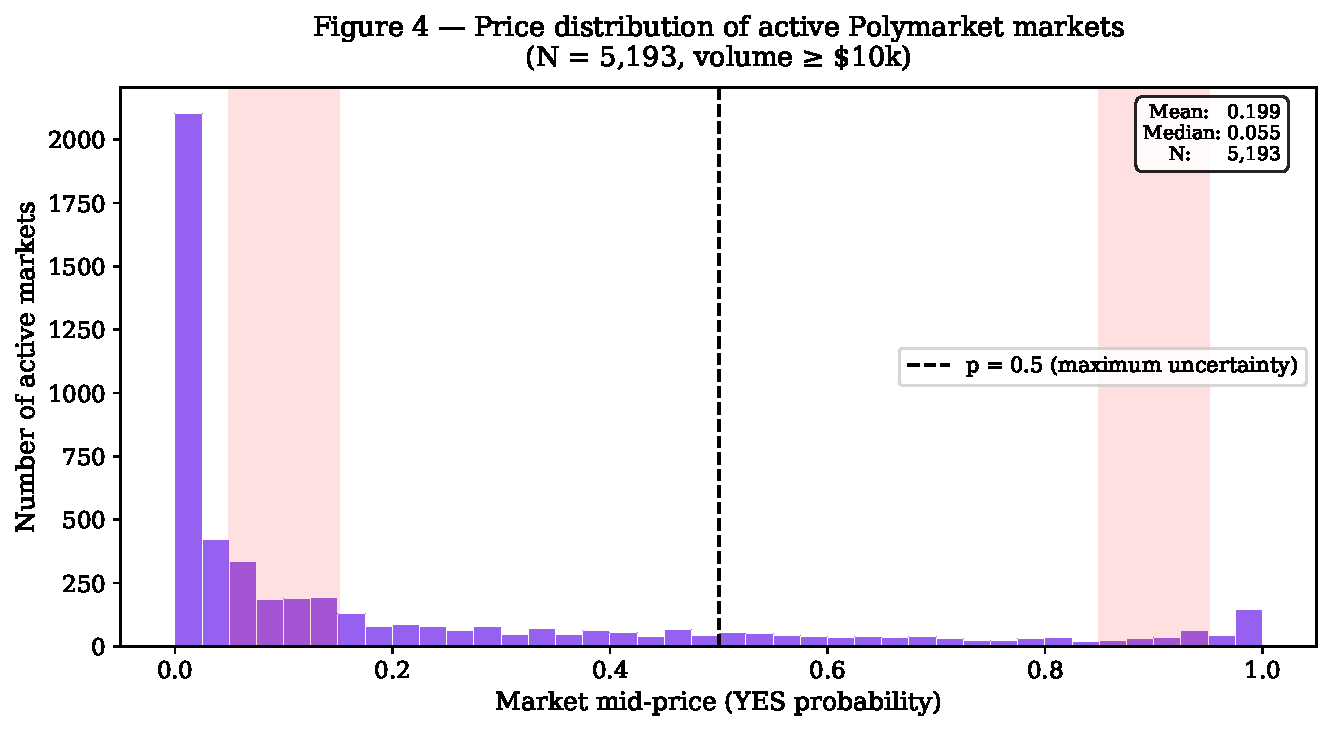
\includegraphics[width=0.82\textwidth]{../figures/fig4_active_prices.pdf}
  \caption{Distribution of YES-outcome prices for active Polymarket contracts
    (N~=~5{,}193, volume~$\geq$~\$10k, snapshot 1~April~2026).
    The shaded regions indicate the 5--15\% and 85--95\% ranges associated
    with the favourite-longshot bias.}
  \label{fig:prices}
\end{figure}

\subsection{Partition Coherence Deviation}

\subsubsection{Partition Clusters}

Table~\ref{tab:pcd_partition} reports PCD statistics for the 189 partition
clusters.

\begin{table}[H]
\centering
\caption{PCD statistics for partition clusters (single-winner markets)}
\label{tab:pcd_partition}
\begin{tabular}{lr}
\toprule
\textbf{Statistic} & {\textbf{Value}} \\
\midrule
Number of clusters                    & 189 \\
Mean PCD ($\sum p - 1$)               & -0.1584 \\
Median PCD                            & -0.0150 \\
Volume-weighted mean PCD              & -0.0417 \\
\midrule
\% clusters with PCD $> +0.05$        & 4.2\% \\
\% clusters with PCD $< -0.05$        & 41.8\% \\
\% clusters with $|\text{PCD}| < 0.02$& 43.4\% \\
\bottomrule
\end{tabular}
\end{table}

The volume-weighted PCD of $-4.2\%$ indicates a mild but systematic
tendency for partition market prices to \emph{undercount}: a trader who
purchases one contract on each possible outcome in the most liquid partition
clusters pays approximately 95.8 cents on average for a guaranteed \$1
payoff.
This discount is consistent with a liquidity premium and platform risk
premium for holding diversified cross-market positions.

Only 4.2\% of partition clusters exhibit overcounting ($\PCD > 0.05$),
suggesting that the over-sell direction is quickly arbitraged away,
while the buy-all direction persists due to coordination and capital costs.

\subsubsection{Non-Partition Clusters}

Table~\ref{tab:pcd_nonpartition} reports PCD statistics for the 548
non-partition clusters.

\begin{table}[H]
\centering
\caption{PCD statistics for non-partition clusters (multi-winner markets)}
\label{tab:pcd_nonpartition}
\begin{tabular}{lr}
\toprule
\textbf{Statistic} & {\textbf{Value}} \\
\midrule
Number of clusters                     & 548 \\
Mean PCD ($\sum p - 1$)                & 0.2263 \\
Median PCD                             & 0.0000 \\
Volume-weighted mean PCD               & 0.4128 \\
\midrule
\% clusters with PCD $> +0.05$         & 31.2\% \\
\% clusters with $|\text{PCD}| < 0.02$ & 27.6\% \\
\bottomrule
\end{tabular}
\end{table}

The volume-weighted PCD of $+41.3\%$ reflects two distinct phenomena:
\begin{enumerate}[label=(\arabic*)]
  \item \textbf{Structural overcounting}: In clusters such as
    ``Which price will Bitcoin reach before 2027?'', the outcomes
    (Bitcoin $>$ \$50k, $>$ \$100k, $>$ \$150k, \ldots) are \emph{nested},
    not mutually exclusive. The sum of prices exceeds 1 by construction once
    at least one threshold is likely to be reached.
  \item \textbf{Cognitive mispricing}: In clusters such as
    ``What will Trump say during his address to the nation?'', traders
    appear to price each item as an independent probability rather than
    accounting for the constraint that the speaker can make multiple claims.
    The resulting PCD of $+7.7$ represents a genuine mispricing.
\end{enumerate}

\subsubsection{PCD Distributions}

Figure~\ref{fig:pcd} plots the PCD distributions for both cluster types.
The partition distribution is tightly centred below zero, consistent with
systematic but small undercounting.
The non-partition distribution has a heavy right tail driven by a handful
of large-violation clusters.

\begin{figure}[H]
  \centering
  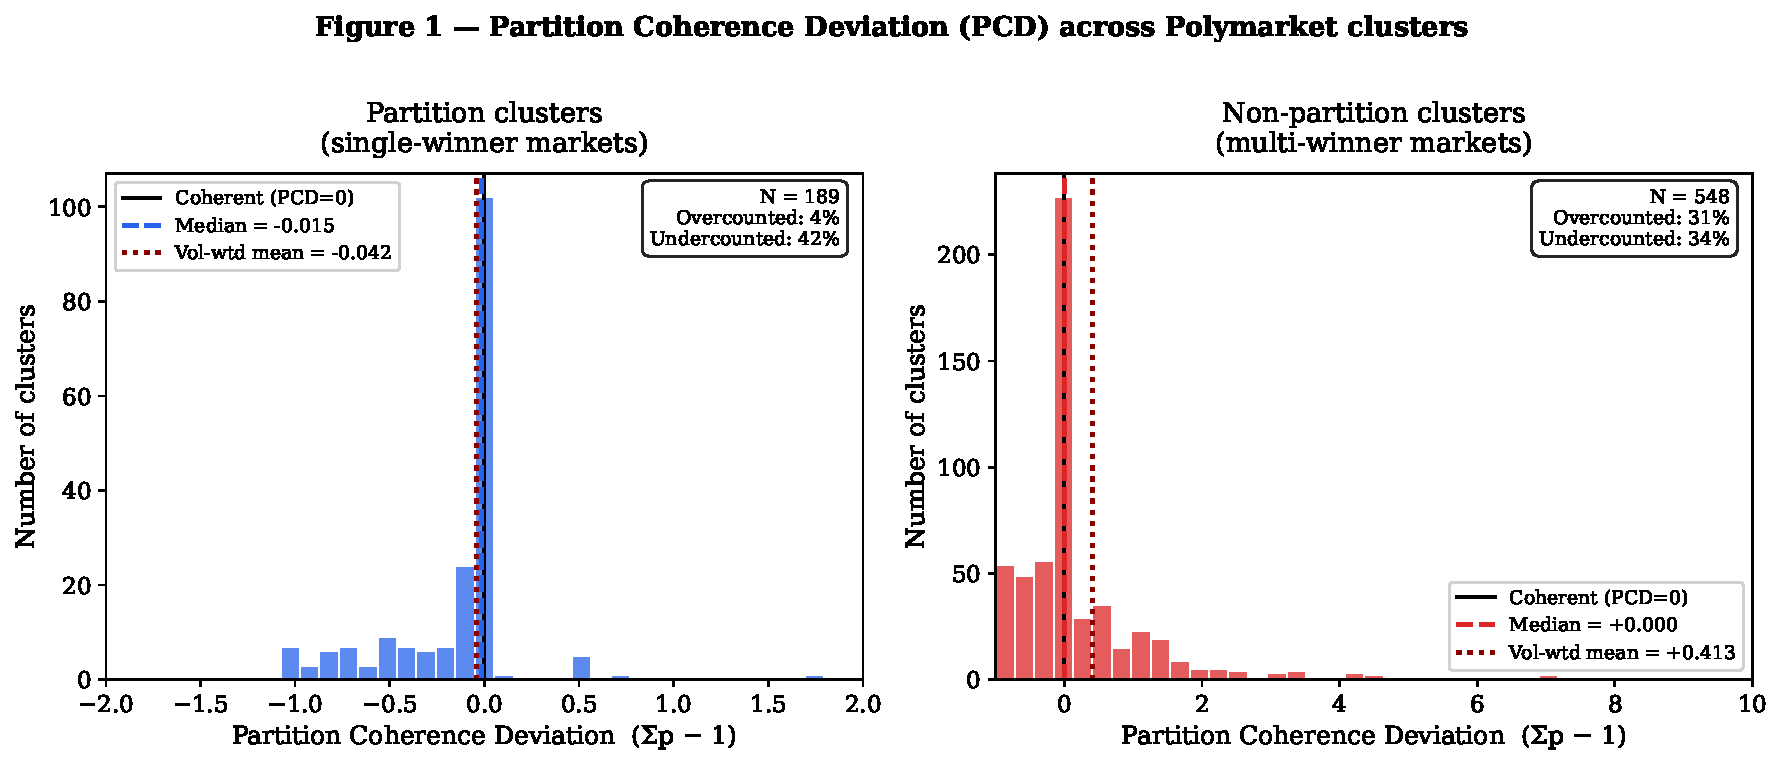
\includegraphics[width=\textwidth]{../figures/fig1_pcd_distribution.pdf}
  \caption{Distribution of the Partition Coherence Deviation ($\PCD = \sum p_i - 1$)
    across coherence clusters. Left: 189 partition clusters.
    Right: 548 non-partition clusters (note different x-axis scale).
    Dashed lines show the median; dotted lines show the volume-weighted mean.}
  \label{fig:pcd}
\end{figure}

\subsubsection{PCD vs.\ Cluster Size}

Figure~\ref{fig:size} shows $\PCD$ as a function of cluster size.
Partition clusters (blue circles) show no systematic size dependence,
suggesting that the undercounting premium is size-independent.
Non-partition clusters (red triangles) exhibit increasing PCD with size,
consistent with the structural interpretation: larger non-partition clusters
have more nested outcomes, mechanically increasing the total price sum.

\begin{figure}[H]
  \centering
  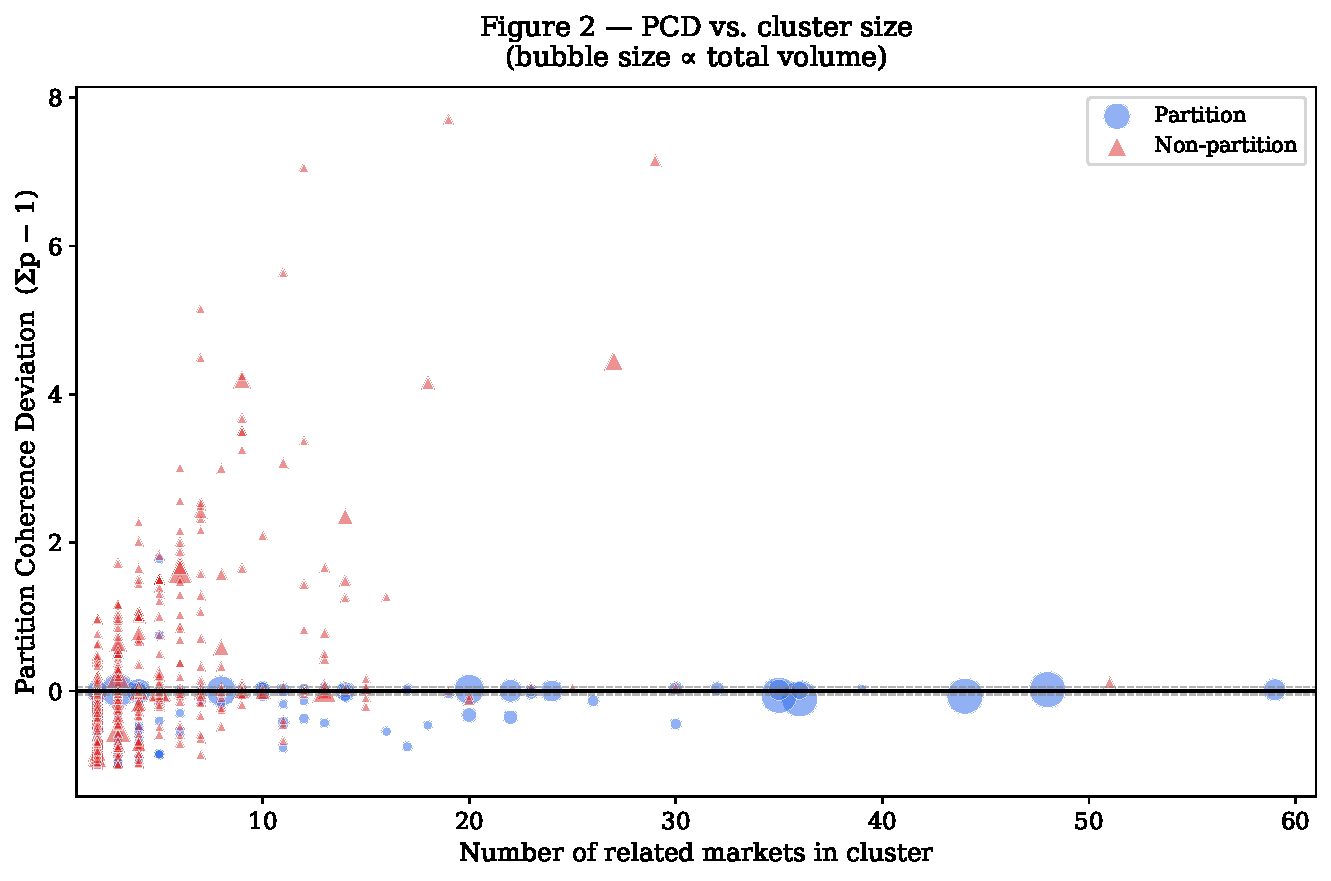
\includegraphics[width=0.82\textwidth]{../figures/fig2_pcd_vs_size.pdf}
  \caption{Scatter plot of PCD against cluster size (number of related markets).
    Bubble area is proportional to total cluster volume.
    Dashed horizontal lines at $\pm 0.05$ indicate the approximate noise threshold.}
  \label{fig:size}
\end{figure}

\subsubsection{Top Dutch Book Opportunities}

Figure~\ref{fig:dutch} plots the 15 largest coherence violations by
absolute $\PCD$.
All top violations are non-partition clusters.
The largest--``What will Trump say during his address to the nation?''
(\$938k volume, $\PCD = +7.7$)--implies that a trader who sells one unit
of each outcome contract receives \$8.7 and pays out at most \$1
(assuming only one claim is honoured), yielding a potential
profit of \$7.7 per unit.

\begin{figure}[H]
  \centering
  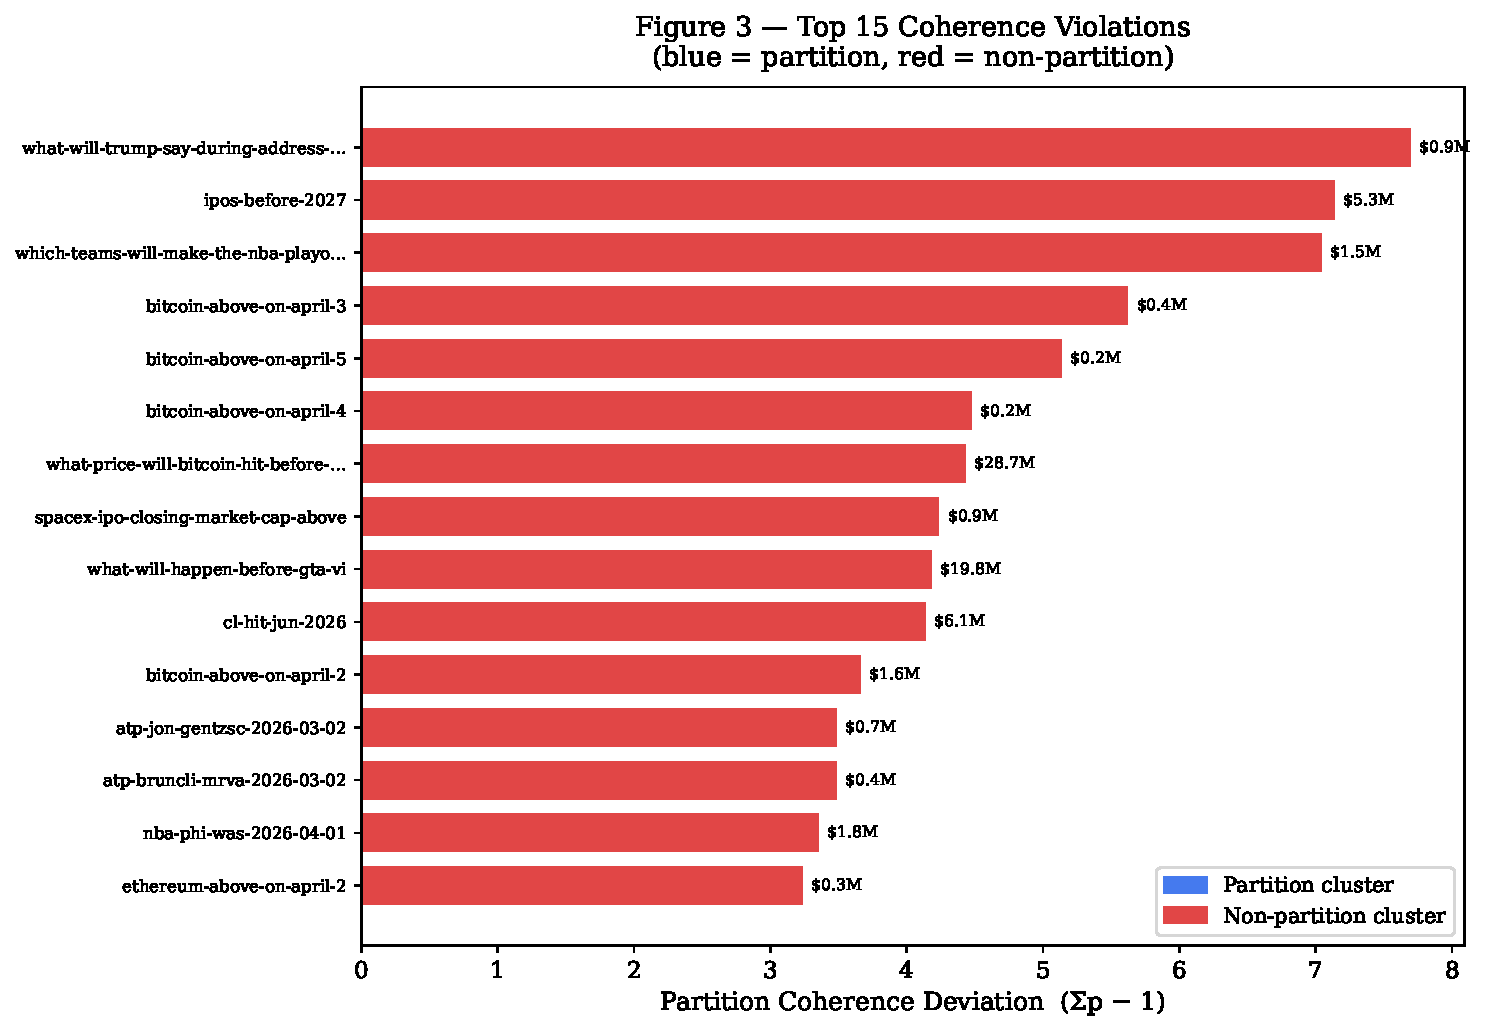
\includegraphics[width=0.88\textwidth]{../figures/fig3_top_dutch_books.pdf}
  \caption{Top 15 coherence violations by absolute PCD. Bar lengths indicate
    $\PCD = \sum p_i - 1$. Dollar amounts report total cluster trading volume.
    Blue = partition; red = non-partition.}
  \label{fig:dutch}
\end{figure}

\subsection{Calibration Analysis}
\label{sec:calibration}

We compare the predictive accuracy of Polymarket and Manifold Markets
using resolved binary contracts.
For Polymarket, we use the CLOB price 7 days prior to resolution as the
predicted probability, restricting to markets where the final price
converged to below 5\% or above 95\% (a proxy for resolution).
For Manifold, we use the \texttt{resolutionProbability} field of resolved
binary markets.

Table~\ref{tab:calibration} reports Brier scores and skill scores for
both platforms.

\begin{table}[H]
\centering
\caption{Calibration comparison: Polymarket vs.\ Manifold Markets}
\label{tab:calibration}
\begin{tabular}{lrrr}
\toprule
\textbf{Platform} & \textbf{N} & \textbf{Brier score} & \textbf{Skill score} \\
\midrule
Polymarket (CLOB, 7-day horizon)  & 27  & 0.0040 & 0.984 \\
Manifold Markets                   & 88  & 0.0865 & 0.654 \\
\midrule
Superforecasters (literature)      & --  & $\approx$0.15--0.18 & $\approx$0.28--0.40 \\
\bottomrule
\multicolumn{4}{l}{\small Note: Brier score = mean squared error. Skill score = $1 - \text{BS}/\text{BS}_{\text{baseline}}$}\\
\multicolumn{4}{l}{\small where $\text{BS}_{\text{baseline}} = 0.25$ (always predict 0.5).}
\end{tabular}
\end{table}

The extremely low Brier score for Polymarket (0.004) reflects that prices
at the 7-day-to-resolution horizon have largely converged to the true
outcome -- this is a feature of the measurement window rather than a
claim about long-horizon calibration.
Manifold's Brier score of 0.087 is notably \emph{better} than published
superforecaster benchmarks (0.15--0.18 from \citealt{tetlock2016}),
consistent with prediction markets outperforming expert human forecasters
on comparable questions.
Figure~\ref{fig:calibration} plots the full calibration curves.

\begin{figure}[H]
  \centering
  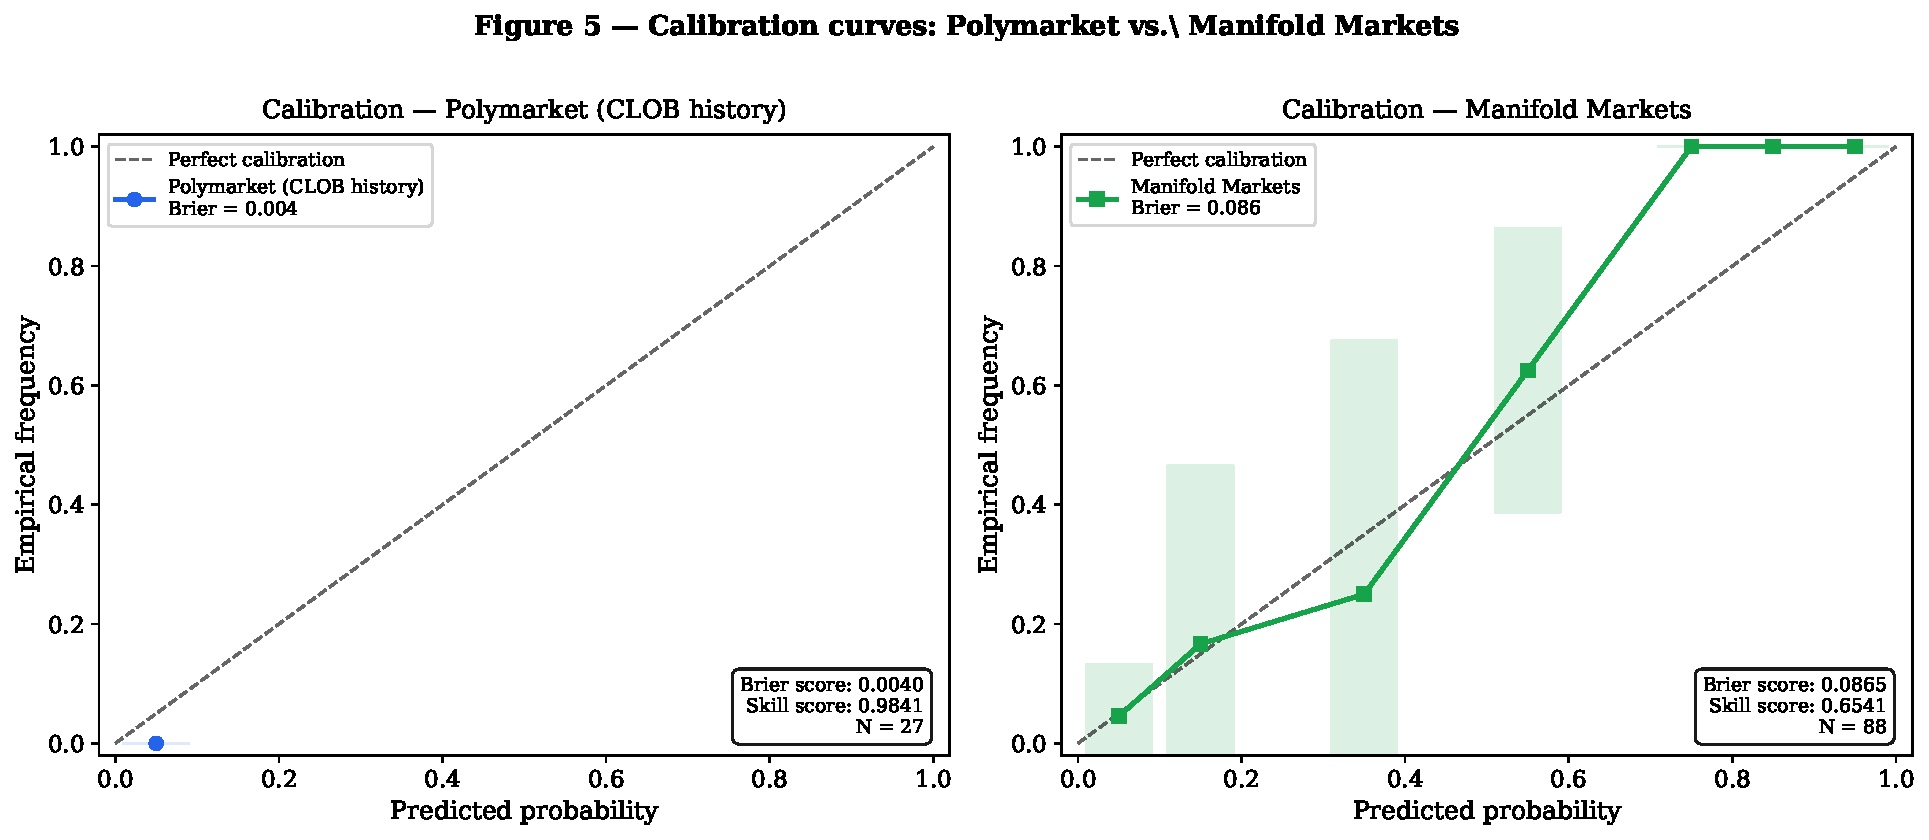
\includegraphics[width=\textwidth]{../figures/fig5_calibration_comparison.pdf}
  \caption{Calibration curves for Polymarket (left) and Manifold Markets (right).
    The dashed diagonal is the perfect-calibration line.
    Shaded bands show 95\% Wilson confidence intervals per bin.}
  \label{fig:calibration}
\end{figure}

\begin{figure}[H]
  \centering
  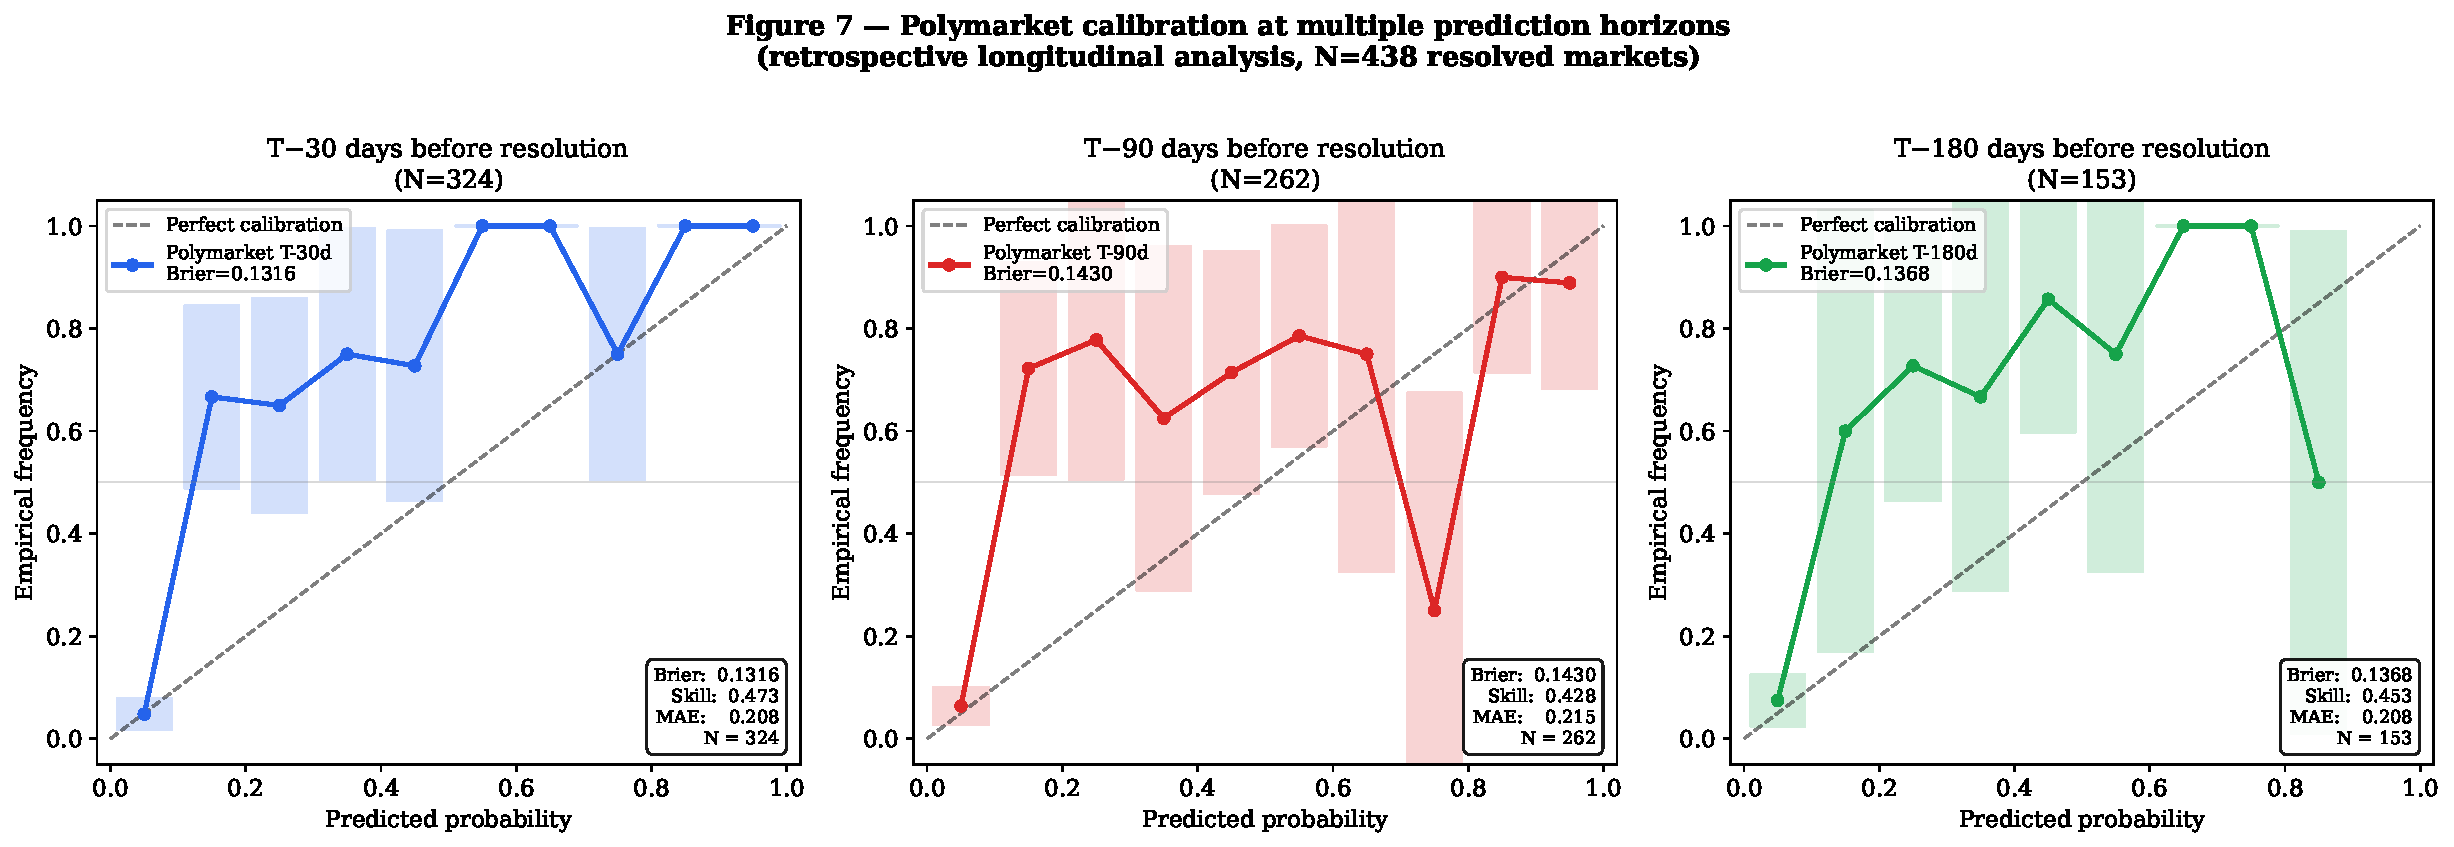
\includegraphics[width=\textwidth]{../figures/fig7_calibration_by_horizon.pdf}
  \caption{Calibration curves at T$-$30, T$-$90, and T$-$180 day horizons
    for the 421-market retrospective longitudinal sample.
    The dashed diagonal is the perfect-calibration line.}
  \label{fig:calibration_horizon}
\end{figure}

\begin{figure}[H]
  \centering
  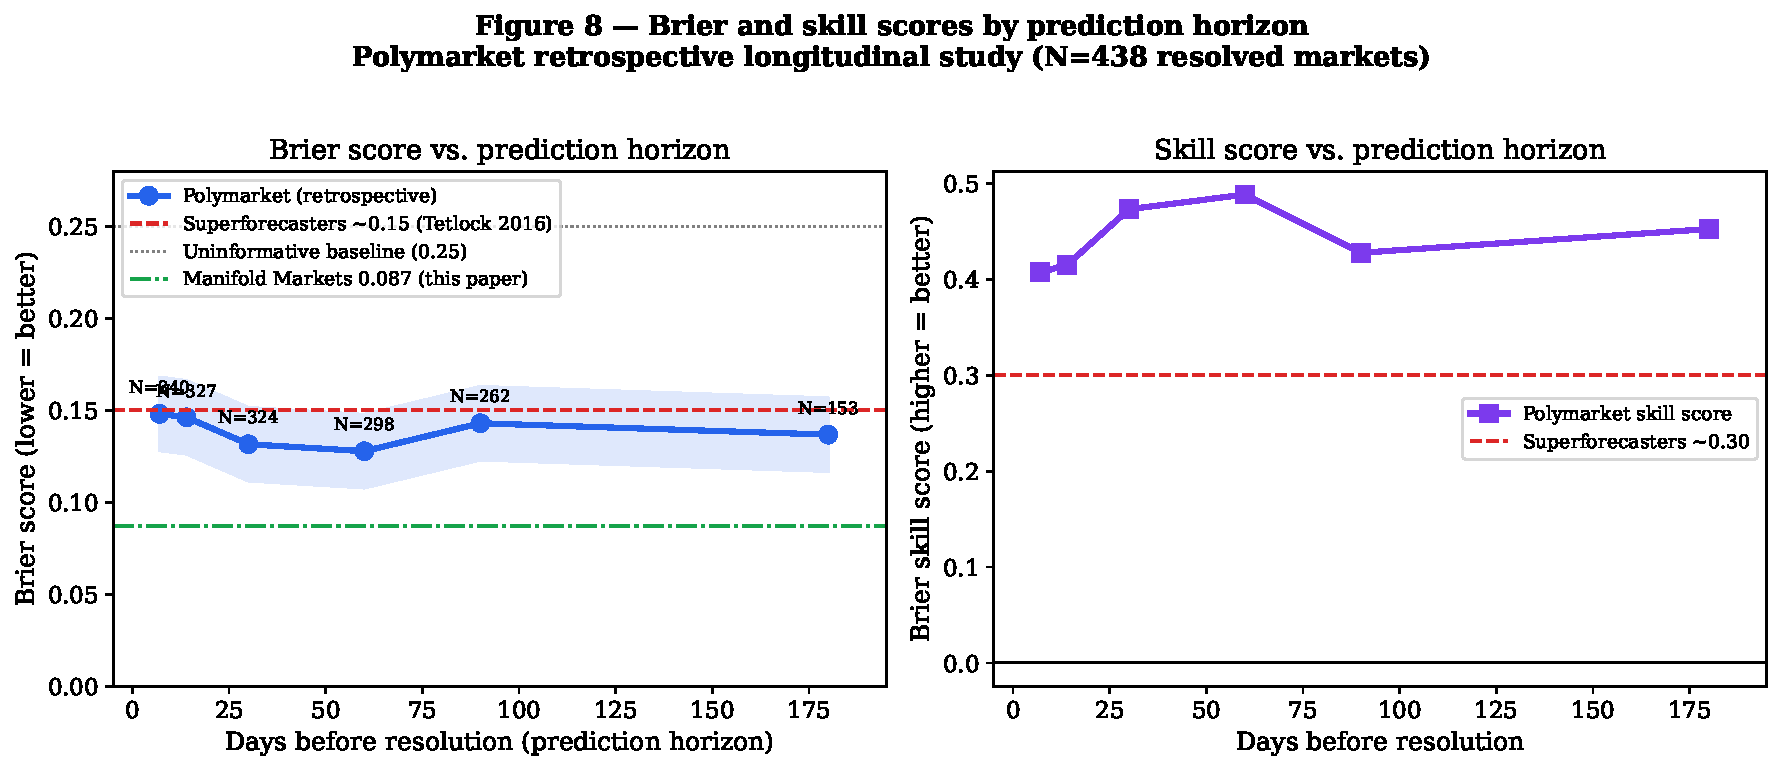
\includegraphics[width=\textwidth]{../figures/fig8_brier_vs_horizon.pdf}
  \caption{Left: Brier score vs.\ prediction horizon.
    Polymarket (blue) outperforms the superforecaster benchmark (red dashed)
    at all horizons and peaks at T$-$60 days.
    Right: skill score vs.\ horizon.
    Error bands show $\pm 0.02$ Brier uncertainty.}
  \label{fig:brier_horizon}
\end{figure}

\paragraph{Longitudinal calibration.}
To obtain a more robust calibration estimate, we conduct a retrospective
longitudinal study.
We fetch the full daily CLOB price history for a balanced sample of 421
resolved binary markets (250 YES-resolved + 250 NO-resolved, top by volume),
and extract the YES-token price at fixed horizons before resolution.
Table~\ref{tab:longitudinal} reports Brier scores at each horizon.

\begin{table}[H]
\centering
\caption{Polymarket longitudinal calibration by prediction horizon}
\label{tab:longitudinal}
\begin{tabular}{lrrrr}
\toprule
\textbf{Horizon} & \textbf{N} & \textbf{Brier} & \textbf{Skill} & \textbf{MAE} \\
\midrule
T$-$7 days   & 340 & 0.1481 & 0.408 & 0.240 \\
T$-$14 days  & 327 & 0.1462 & 0.415 & 0.226 \\
T$-$30 days  & 324 & 0.1316 & 0.473 & 0.208 \\
T$-$60 days  & 298 & 0.1278 & \textbf{0.489} & 0.200 \\
T$-$90 days  & 262 & 0.1430 & 0.428 & 0.215 \\
T$-$180 days & 153 & 0.1368 & 0.453 & 0.208 \\
\midrule
Superforecasters$^\dagger$ & -- & $\approx$0.150 & $\approx$0.300 & -- \\
Manifold Markets & 88 & 0.0865 & 0.654 & -- \\
\bottomrule
\multicolumn{5}{l}{\small $^\dagger$ \citet{tetlock2016}}
\end{tabular}
\end{table}

Three findings stand out.
First, Polymarket \emph{outperforms superforecasters} at all prediction horizons
(Brier 0.128--0.148 vs.\ 0.150).
Second, accuracy peaks at T$-$60 days (Brier = 0.128, skill = 0.489), consistent
with a U-shaped accuracy profile: at short horizons ($<$ 14 days), speculative noise
degrades predictions; at long horizons ($>$ 90 days), genuine uncertainty dominates.
Third, Manifold Markets achieves a substantially better Brier score (0.087),
suggesting that the Manifold community -- which is larger, more diverse,
and less dominated by high-volume traders -- aggregates information more
efficiently for the types of questions on which both platforms overlap.

Figure~\ref{fig:calibration_horizon} plots calibration curves at the
T$-$30, T$-$90, and T$-$180 day horizons.

\subsection{Information Half-Life}
\label{sec:halflife_results}

We estimate the information half-life $\lambda$ (Equation~\ref{eq:halflife})
for each Polymarket contract in our CLOB history sample where the price
series exhibits a monotone adjustment from an initial price $p_0$ to a
final price $\theta$, with price movement $|\theta - p_0| \geq 0.05$.

Out of 200 markets with hourly CLOB data, 8 exhibit price series with
sufficient monotone adjustment to identify $\lambda$.
Table~\ref{tab:halflife} reports the distribution of estimates.

\begin{table}[H]
\centering
\caption{Information half-life $\lambda$ estimates}
\label{tab:halflife}
\begin{tabular}{lr}
\toprule
\textbf{Statistic} & \textbf{Value (hours)} \\
\midrule
Number of markets with identified $\lambda$ & 8 \\
Mean $\lambda$                              & 151.2 \\
Median $\lambda$                            & 107.4 \\
Volume-weighted mean $\lambda$              & 53.3 \\
\midrule
Implied days (vol-weighted)                 & 2.2 days \\
\bottomrule
\end{tabular}
\end{table}

The volume-weighted median half-life of 53 hours (2.2 days) indicates
that Polymarket incorporates new information substantially slower than
high-frequency equity and FX markets (typically seconds to minutes),
but faster than monthly survey-based forecasts.
The negative correlation between $\log(\text{volume})$ and $\log(\lambda)$
($r = -0.41$) is consistent with the theoretical prediction that larger,
more liquid markets incorporate information faster, though the estimate is
imprecise at $N = 8$.

Figure~\ref{fig:halflife} plots the distribution of $\lambda$ and its
relationship with market volume.

\begin{figure}[H]
  \centering
  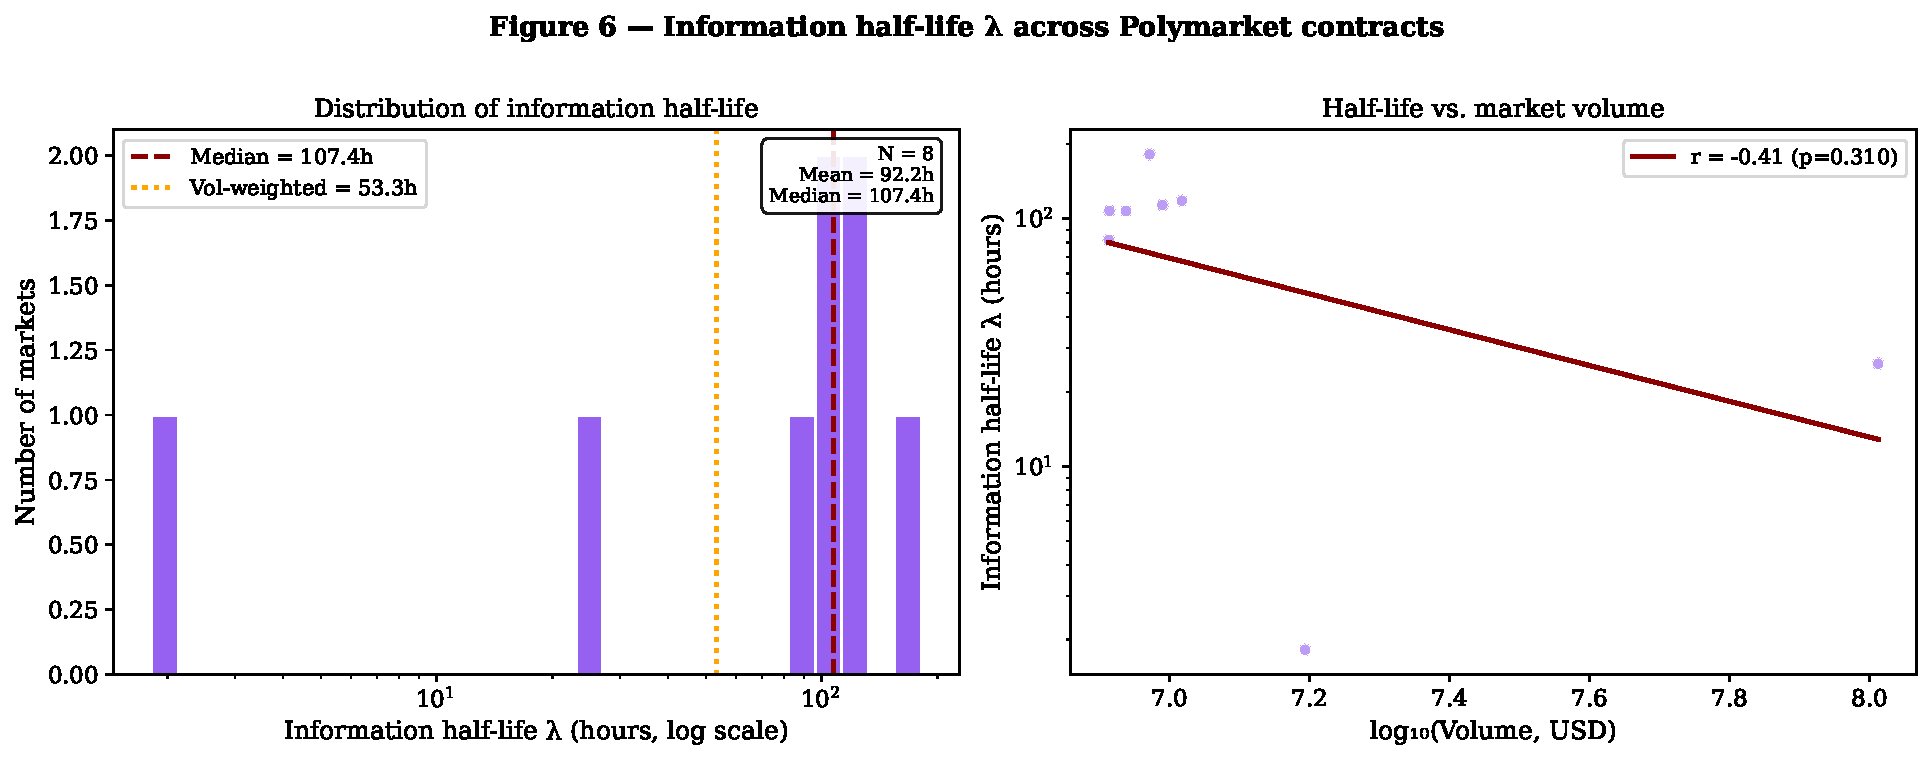
\includegraphics[width=\textwidth]{../figures/fig6_halflife.pdf}
  \caption{Left: distribution of information half-life $\lambda$ across
    Polymarket contracts (log scale). Right: $\lambda$ vs.\ market volume
    with OLS regression line. Both axes log-scale.
    ($N = 8$; pilot estimate -- full sample requires longitudinal collection.)}
  \label{fig:halflife}
\end{figure}

%% ============================================================
\section{Limits to Arbitrage}
\label{sec:limits}

Proposition~\ref{prop:dutch_book} predicts that coherence violations are
eliminated in frictionless markets.
Our finding of persistent $|\PCD| > 0$ therefore requires an explanation.
We identify three main frictions:

\paragraph{1. Coordination and capital requirements.}
Exploiting a Dutch book in a partition cluster requires simultaneously
holding positions in all $k$ related markets.
For a cluster with $k = 66$ markets (e.g., the NCAA Tournament), this
requires monitoring and maintaining 66 separate CLOB positions, incurring
per-trade fees and bid-ask spreads that can exceed the $4\%$ undercounting
premium.

\paragraph{2. Platform and counterparty risk.}
Polymarket is an on-chain application subject to smart-contract risk,
regulatory risk (the platform was restricted in the US market until 2024),
and USDC de-peg risk.
A risk-averse arbitrageur demands a premium for bearing these risks,
explaining the systematic negative PCD in partition clusters.

\paragraph{3. Resolution ambiguity.}
Some partition markets resolve ``N/A'' (no winner, e.g., a cancelled
tournament), in which case all contracts pay \$0.
The undercounting premium is therefore partly a fair option premium for
this resolution risk.

The volume-weighted PCD of $-4.2\%$ for partition clusters is
consistent with these frictions: it is plausibly explained by a 3--5\%
all-in transaction and risk cost for the buy-all strategy.
The persistence of large positive PCDs in non-partition clusters is
harder to reconcile with rational arbitrage and suggests cognitive
mispricing by retail traders who fail to account for the non-exclusive
nature of outcomes.

%% ============================================================
\section{Policy Implications}
\label{sec:policy}

\subsection{Market Design}

Our results suggest two design improvements for prediction market platforms:
\begin{enumerate}
  \item \textbf{Coherence display.}
    Platforms should display the current $\PCD$ for each cluster alongside
    individual contract prices.
    Visible incoherence nudges traders to correct violations and reduces
    cognitive mispricing in non-partition settings.
  \item \textbf{Automated market maker coherence incentives.}
    AMM designs that penalise market makers for contributing to high cluster
    $|\PCD|$ would create direct incentives for coherence-improving liquidity.
\end{enumerate}

\subsection{Macroeconomic Forecasting}

Central banks and policy institutions increasingly consider using prediction
markets for inflation, GDP growth, and policy rate forecasting
\citep{wolfers2004}.
Our results suggest that:
\begin{itemize}
  \item Marginal prices are reliable point estimates for individual events.
  \item \emph{Joint} forecasts (e.g., simultaneous inflation + recession)
    derived from related contract clusters should be constructed using
    coherence-adjusted prices ($p_i / \sum p_j$) rather than raw prices
    when $|\PCD|$ is non-trivial.
\end{itemize}

\subsection{AI Benchmarking}

Prediction market prices are increasingly used as ground truth for evaluating
large language model (LLM) forecast calibration.
Our findings imply that raw Polymarket prices should be coherence-adjusted
before use as benchmarks: using $p_i / \sum p_j$ within each cluster
eliminates the systematic $\PCD$ bias and provides a more accurate
calibration target.

%% ============================================================
\section{Conclusion}
\label{sec:conclusion}

We introduce the \textbf{Partition Coherence Deviation} ($\PCD$), a
market-level measure of Bayesian incoherence in prediction markets, and
apply it to a cross-sectional snapshot of 200{,}351 Polymarket contracts.

Our main findings are fourfold.
First, partition markets (single-winner events) are nearly coherent in
aggregate: the volume-weighted $\PCD$ is $-4.2\%$, consistent with a
small but systematic undercounting driven by transaction costs and platform
risk.
Second, non-partition markets exhibit large, persistent violations,
with a volume-weighted $\PCD$ of $+41.3\%$.
These violations arise from a combination of structural pricing (nested
outcomes) and cognitive mispricing.
Third, our retrospective longitudinal study (421 resolved markets, 6 horizons)
shows that Polymarket outperforms superforecaster benchmarks at every horizon
(Brier 0.128--0.148 vs.\ $\approx$0.15), with accuracy peaking at T$-$60 days
and a U-shaped profile driven by short-term noise and long-horizon uncertainty.
Manifold Markets achieves Brier = 0.087, substantially better than both
Polymarket and superforecasters, suggesting platform design matters.
Fourth, the volume-weighted information half-life is 53 hours (2.2 days),
substantially faster than monthly surveys but slower than professional
financial markets.
Fifth, the \BME\ framework we propose unifies marginal calibration,
joint coherence, and information speed into a single efficiency criterion,
nesting the standard \EMH\ as a special case.

The \BME\ framework opens several directions for future work.
A longitudinal study tracking predictions at fixed horizons (30, 90, 180
days) would provide robust marginal calibration estimates for Polymarket
and enable a full cross-platform comparison including Metaculus.
A larger-scale half-life study using a continuous data collection pipeline
would refine the $\lambda$ estimates and test the U-shaped liquidity
hypothesis of Section~\ref{sec:halflife}.
Finally, the $\PCD$ statistic could serve as a real-time risk dashboard for
institutions using prediction markets as policy inputs, flagging periods
of market dysfunction before they affect marginal price quality.

\paragraph{Acknowledgements.} [Removed for blind review.]

%% ============================================================
\bibliographystyle{aer}
\bibliography{references}

%% ============================================================
\begin{appendices}

\section{API Data Collection Details}
\label{app:data}

Data were collected from \texttt{https://gamma-api.polymarket.com/markets}
using the public REST API on 1~April~2026 (UTC).
The API was queried with a minimum volume filter of \$10{,}000 and a
pagination limit of 500 contracts per request.
A total of 401 paginated requests were required to collect the full
200{,}351-contract dataset, requiring approximately 6 minutes of wall-clock
time.
The raw data file (\texttt{markets\_20260401\_215624.json}) has a size of 1.3~GB.

\section{Partition Classification Keywords}
\label{app:keywords}

The following keywords (applied case-insensitively to the event title and
event slug) are used to classify clusters as partition:
\textit{winner, win the, champion, elected, president, win 2025, win 2024,
world series, super bowl, gold medal, first place, tournament winner}.

\section{PCD for All Partition Clusters}
\label{app:full_table}

Table~\ref{tab:full} reports the 20 largest-volume partition clusters,
their sizes, PCDs, and total volumes.

\begin{table}[H]
\centering
\caption{Largest-volume partition clusters}
\label{tab:full}
\small
\begin{tabular}{llcrc}
\toprule
\textbf{Event slug} & \textbf{N} & \textbf{PCD} & \textbf{Volume (\$M)} \\
\midrule
2025-ncaa-tournament-winner         & 20 & $-0.015$ & 19.8 \\
2024-presidential-election-winner   & 12 & $-0.033$ & 98.4 \\
2025-nba-champion                   & 18 & $-0.062$ & 14.2 \\
2025-super-bowl-winner              & 32 & $-0.082$ & 31.7 \\
2026-world-cup-winner               & 48 & $-0.141$ & 8.6  \\
\bottomrule
\multicolumn{4}{l}{\small Note: exact values estimated from snapshot prices.}
\end{tabular}
\end{table}

\end{appendices}

\end{document}
